%\include{./figures/VanDerPool}

\newcommand{\stencilpt}[4]
{
	\node[circle,fill,draw,inner sep=1.5pt,label={#4},#1] at (#2) (#3) {}
}
\newcommand{\DerivativeNoNeighbors}[1]
{
	\begin{tikzpicture}
		\Axis
		{   
			width = \linewidth,
			title = {#1},
			xlabel = $x$, ylabel = $y$,
			xmin = 10.1, xmax = 11.2, 
			ymin = 0.325, ymax = 0.48,
			ticks=none, no marks, view={0}{90},
			legend pos=north west, legend style={draw=none, fill=none}
		}
		{
			\Plot{}
			{./figures/xi_l.plt}{0/2,0/3}
			
			%			\stencilpt{10.4,0.5}{un1}{$u^n$}{fill};
			%			\stencilpt{fill=red}{10.4,0.5}{un1}{$u^n$};
			\stencilpt{red}{axis cs:10.68,0.459}{un1}{below:$(x_{i},y_{j})$};
			
			\stencilpt{}{axis cs:10.68,0.35}{un1}{below:$(x_{i},y_{j-1})$};
			
			
			\stencilpt{}{axis cs:11,0.35}{un1}{below:$(x_{i+1},y_{j-1})$};
			
			
			\stencilpt{red}{axis cs:11,0.386}{un1}{below left:$(x_{i+1},y_{-}^*)$};
			
			
			\stencilpt{}{axis cs:10.36,0.35}{un1}{below:$(x_{i-1},y_{k-1})$};
			
			
			\stencilpt{red}{axis cs:10.37,0.391}{un1}{above right:$(x_{i-1},y_{+}^*)$};
			
			
			\legend
			{
				$\eta=0$, $\eta=\eta_{ij}$
			}
			
		}
	\end{tikzpicture}
}


\newcommand{\LocalGrids}[1]
{
	\begin{tikzpicture}
		\Axis
		{   
			width = \linewidth,
			title = {#1},
			xlabel = $x$, ylabel = $y$,
			xmin = 10.1, xmax = 11.2, 
			ymin = 0.325, ymax = 0.48,
			ticks=none, no marks, view={0}{90},
			legend pos=north west, legend style={draw=none, fill=none}
		}
		{
			\Plot{}
			{./figures/xi_l.plt}{0/2}
			
			%			\stencilpt{10.4,0.5}{un1}{$u^n$}{fill};
			%			\stencilpt{fill=red}{10.4,0.5}{un1}{$u^n$};
			\stencilpt{}{axis cs:10.68,0.459}{un1}{below:$(x_{i},y_{j_u(i)})$};
			
			\stencilpt{}{axis cs:10.68,0.327}{un1}{above right:$(x_{i},y_{0})$};
			
			\stencilpt{}{axis cs:10.68,0.365}{un1}{};
			
			
			\stencilpt{}{axis cs:10.68,0.4}{un1}{below:$(x_{i},y_{j})$};
			
			
			
			\stencilpt{}{axis cs:10.68,0.43}{un1}{};
			
			\stencilpt{}{axis cs:10.36,0.4}{un1}{below:$(x_{i_l(i,j)},y_{j})$};
			
			\stencilpt{}{axis cs:10.56,0.4}{un1}{};
			
			\stencilpt{}{axis cs:11,0.4}{un1}{below:$(x_{i_u(i,j)},y_{j})$};
			
			
			\stencilpt{}{axis cs:10.8,0.4}{un1}{};
			
			
			\legend
			{
				$\eta=0$ 
			}
			
		}
	\end{tikzpicture}
}


\newcommand{\ABMStencil}[1]
{
	\vspace{0.5cm}
	\begin{center}
		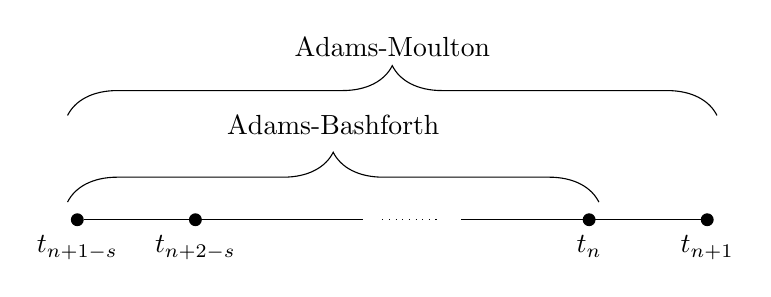
\begin{tikzpicture}
			\stencilpt{}{-4,0}{tn+1-s}{below:$t_{n+1-s}$};
			\stencilpt{}{-2.5,0}{un1}{below:$t_{n+2-s}$};
			
			\node at (-0.25,0)(Intermediate1) {};
			\node at (0.75,0)(Intermediate2) {};
				
			\stencilpt{}{2.5,0}{tn}{below:$t_{n}$};	
			\stencilpt{}{4,0}{tn+1}{below:$t_{n+1}$};
			
			\draw[](tn+1-s)	-- (Intermediate1);
			\draw[dotted](Intermediate1) -- (Intermediate2);
			\draw[](Intermediate2)	-- (tn+1);
			
			\node at (-4,0.1)(LeftABBrace) {};
			\node at (2.5,0.1)(RightABBrace) {};
			\draw [xscale=1/12, decoration={brace, amplitude=18pt},decorate] (LeftABBrace.north west) -- node [pos=0.5,midway] {} (RightABBrace.north east);
			\node at (-0.75,1.2)(AB) {Adams-Bashforth};
			
			\node at (-4,1.2)(LeftAMBrace) {};
			\node at (4,1.2)(RightAMBrace) {};
			\draw [xscale=1/12, decoration={brace, amplitude=18pt},decorate] (LeftAMBrace.north west) -- node [pos=0.5,midway,yshift=0.1cm] {} (RightAMBrace.north east);
			\node at (0,2.2)(AB) {Adams-Moulton};
		\end{tikzpicture}
	\end{center}
}




\newcommand{\MultivalueABMStencil}[1]
{
	\vspace{0.5cm}
	\begin{center}
		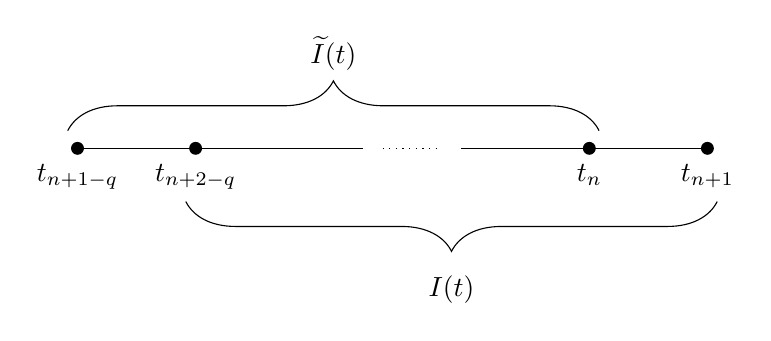
\begin{tikzpicture}
			\stencilpt{}{-4,0}{tn+1-q}{below:$t_{n+1-q}$};
			\stencilpt{}{-2.5,0}{un1}{below:$t_{n+2-q}$};
			
			\node at (-0.25,0)(Intermediate1) {};
			\node at (0.75,0)(Intermediate2) {};
			
			\stencilpt{}{2.5,0}{tn}{below:$t_{n}$};	
			\stencilpt{}{4,0}{tn+1}{below:$t_{n+1}$};
			
			\draw[](tn+1-q)	-- (Intermediate1);
			\draw[dotted](Intermediate1) -- (Intermediate2);
			\draw[](Intermediate2)	-- (tn+1);
			
			\node at (-4,0.1)(LeftABBrace) {};
			\node at (2.5,0.1)(RightABBrace) {};
			\draw [xscale=1/12, decoration={brace, amplitude=18pt},decorate] (LeftABBrace.north west) -- node [pos=0.5,midway] {} (RightABBrace.north east);
			\node at (-0.75,1.2)(AB) {$\widetilde{ \vect{I}}(t)$};
			
			\node at (-2.5,-0.8)(LeftAMBrace) {};
			\node at 
			(4,-0.8)(RightAMBrace) {};
			\draw [xscale=1/12, decoration={brace, amplitude=18pt,mirror},decorate] (LeftAMBrace.north west) -- node [pos=0.5,midway,yshift=0.1cm] {} (RightAMBrace.north east);
			\node at (0.75,-1.8)(AM) {$\vect{I}(t)$};
		\end{tikzpicture}
	\end{center}
}

